\documentclass[10pt,letterpaper]{article}
\usepackage{amsmath}
\usepackage{amsfonts}
\usepackage{amssymb}
\usepackage[utf8]{inputenc}
\usepackage{makeidx}
\usepackage{graphicx}
\usepackage{lmodern}
\usepackage[left=2cm,right=2cm,top=2cm,bottom=2cm]{geometry}
%Used for color for programming language
\usepackage{listings}
\usepackage{color}

\newcommand{\hmwkTitle}{Assignment\ \#4} % Assignment title
\newcommand{\hmwkDueDate}{11:59pm February 27,\ 2018} % Due date
\newcommand{\hmwkClass}{CS 535} % Course/class
\newcommand{\hmwkClassTime}{16:20} % Class/lecture time
\newcommand{\hmwkClassInstructor}{Alexander C. Nwala} % Teacher/lecturer
\newcommand{\hmwkAuthorName}{David Sinclair} % Your name

%----------------------------------------------------------------------------------------
%	TITLE PAGE
%----------------------------------------------------------------------------------------

\title{
\vspace{2in}
\textmd{\textbf{\hmwkClass:\ \hmwkTitle}}\\
\normalsize\vspace{0.1in}\small{Due\ on\ \hmwkDueDate}\\
\vspace{0.1in}\large{\textit{\hmwkClassInstructor\ \hmwkClassTime}}
\vspace{3in}
}
\author{\textbf{\hmwkAuthorName}}


\begin{document}

\maketitle
%----------------------------------------------------------------------------------------
%	TABLE OF CONTENTS
%----------------------------------------------------------------------------------------

%\setcounter{tocdepth}{1} % Uncomment this line if you don't want subsections listed in the ToC

\pagebreak
\tableofcontents
\pagebreak 

%----------------------------------------------------------------------------------------
%	Create colors for scripting 
%----------------------------------------------------------------------------------------


\definecolor{dkgreen}{rgb}{0,0.6,0}
\definecolor{gray}{rgb}{0.5,0.5,0.5}
\definecolor{mauve}{rgb}{0.58,0,0.82}

\lstset{frame=tb,
  language=Python,
  aboveskip=3mm,
  belowskip=3mm,
  showstringspaces=false,
  columns=flexible,
  basicstyle={\small\ttfamily},
  numbers=none,
  numberstyle=\tiny\color{gray},
  keywordstyle=\color{blue},
  commentstyle=\color{dkgreen},
  stringstyle=\color{mauve},
  breaklines=true,
  breakatwhitespace=true,
  tabsize=3
}
%----------------------------------------------------------------------------------------
%	Problem 1 %----------------------------------------------------------------------------------------

\section{Problem 1}
\subsection{Question 1}
The "friendship paradox" (http://en.wikipedia.org/wiki/Friendship\_paradox)
says that your friends have more friends than you do.  \\
\\
1.  Determine if the friendship paradox holds for my Facebook
account.\* Compute the mean, standard deviation, and median of the
number of friends that my friends have.  Create a graph of the
number of friends (y-axis) and the friends themselves, sorted by
number of friends (y-axis).  (The friends don't need to be labeled
on the x\-axis: just f1, f2, f3, ... fn.)  Do include me in the graph
and label me accordingly.\\
\\
\* \= This used to be more interesting when you could more easily download
your friend's friends data from Facebook.  Facebook now requires each
friend to approve this operation, effectively making it impossible.\\
\\
I will upload a csv file of my 2014 friends list on the \#assignment\-4 slack channel\\
\\
\subsection{Answer 1}
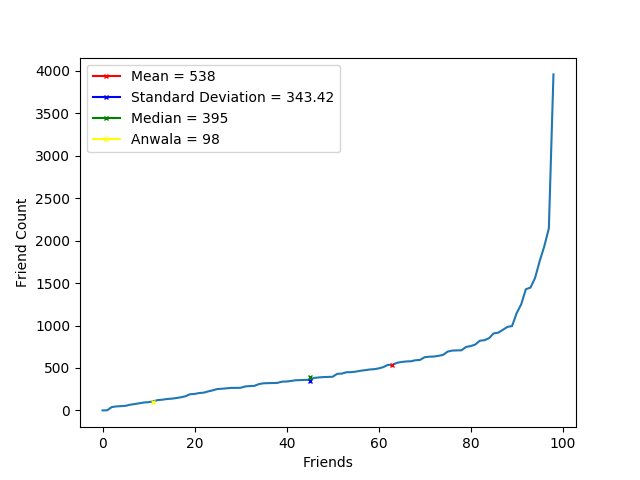
\includegraphics[scale=1]{Question1.png} 
\pagebreak 

%----------------------------------------------------------------------------------------
%	Problem 2
%----------------------------------------------------------------------------------------
\section{Problem 2}
\subsection{Question 2}
2.  Determine if the friendship paradox holds for your Twitter account.
Since Twitter is a directed graph, use "followers" as value you measure
(i.e., "do your followers have more followers than you?").\\
\\
Generate the same graph as in question \#1, and calcuate the same 
mean, standard deviation, and median values.\\
\\
For the Twitter 1.1 API to help gather this data, see:\\
\\
https://developer.twitter.com/en/docs/accounts-and-users/follow-search-get-users/api-reference/get-followers-list\\
\\
If you do not have followers on Twitter (or don't have more than 50),
then use my twitter account "acnwala".\\
\\
\subsection{Answer 2}
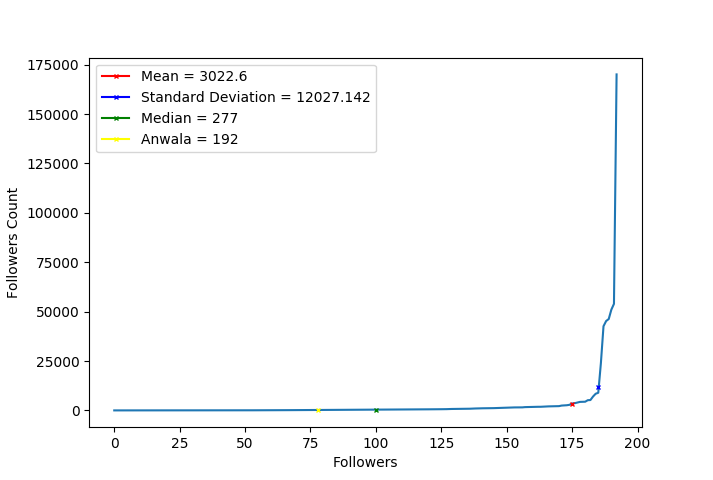
\includegraphics[scale=1]{Question2.png} 

\pagebreak
%----------------------------------------------------------------------------------------
%	Problem 3
%----------------------------------------------------------------------------------------
\section{Problem 3}
\subsection{Question 3}
Extra credit, 3 points:\\
\\
3.  Repeat question \#1, but with your (or a specified) LinkedIn profile.\\
\\
\subsection{Answer 3}


\pagebreak
%----------------------------------------------------------------------------------------
%	Problem 4
%----------------------------------------------------------------------------------------
\section{Problem 4}
\subsection{Question 4}
Extra credit, 1 point:\\
\\
4.  Repeat question \#2, but change "followers" to "following"?  In
other words, are the people I am following following more people?\\
\\
For the Twitter 1.1 API to help gather this data, see:\\
\\
https://developer.twitter.com/en/docs/accounts-and-users/follow-search-get-users/api-reference/get-friends-list\\
\\
\subsection{Answer 4}
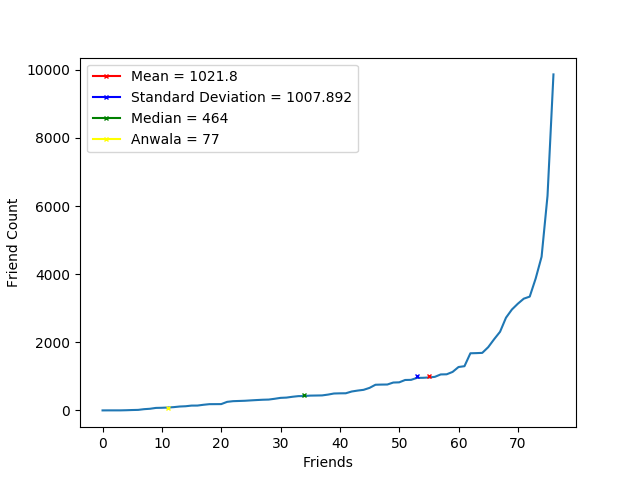
\includegraphics[scale=1]{Question4.png}
\pagebreak

\end{document}
